\chapter{Exploratory Research Design}
\label{chap:exploratoryResearchDesign}

\section{Overview of Approach}
Due to the iterative nature of exploratory work, this paper is not structured by methodology, results, and discussion but progresses iteratively. For our results to be meaningful and to progress in an efficient manner, the research of the paper is structured into multiple experimentation cycles. Each cycle is comprised of:

\begin{enumerate}
    \item Determining Objective(s)
    \item Defining Hypotheses
    \item Build Approach
    \item Present Results
    \item Immediate Discussion
\end{enumerate}

This structure allows for a more flexible approach to the research. It allows us to adapt as new insights are gained and form new hypotheses without compromising the experiment. This supports the dynamic nature of exploratory research, where learning and adaptation are key.

\subsection*{Determining Objective(s)}
The first step in each experimentation cycle is to clearly define what objective we are trying to achieve. This objective, or objectives, guide the research for the cycle, determining which hypotheses are chosen and how to approach the research. Objectives may be refined or adjusted as data is gathered and new insights are formed.

\subsection*{Defining Hypotheses}
As objectives are chosen, we can begin formulating hypotheses we aim to test or explore. We will test these predictions and provide a clear direction for the experimentation and analysis phases. Hypotheses should be specific and should not change as new data is gathered -- for that, we can note down the new questions that arise, which will inform the next research cycle.

\subsection*{Build Approach}
With our objectives and hypotheses defined, this stage will focus on designing and planning our experimentation process. This includes selecting methodologies, defining which data to collect and how, and outlining the analysis techniques to be employed. This approach should be designed to efficiently test and answer the stated hypotheses, achieving the cycle's objectives.

\subsection*{Present Results}
This section presents all results from the experimentation and analysis of said data. The results should be detailed for clear analysis and focused on transparency and reproducibility to support the next discussion phase and future research.

\subsection*{Immediate Discussion}
This final phase is an immediate critical discussion of the derived results. The data provides insights and discusses the implications for the paper's wider research goals. These insights and results feed directly into the design of the next cycle, and the learning gained, in turn, informs how we structure the following objective and approach.


\section{Initial Hypotheses}
We wish to test four main hypotheses in this paper. We discuss the reason for their inclusion, what proving the hypotheses means regarding our research goals, and what contradicting them would indicate.

\subsection{Ping Pong Handover Prevalence}
Ping Pong Handover will be much more prevalent due to the denser configuration of indoor networks.
\begin{itemize}
    \item \textbf{Expectation:} Increased Ping Pong Handovers are anticipated due to the closer proximity of access points and the resulting signal overlap. Small signal fluctuations could result in a handover to a neighbour cell and then immediately back again.
    \item \textbf{Implication:} A higher incidence of Ping Pong Handovers could indicate a need for more careful tuning of handover parameters or even more sophisticated handover algorithms tailored to dense environments - such as a Machine Learning based one.
    \item \textbf{Consideration:} Contradicting this hypothesis may suggest existing handover mechanisms are more effective in dense configurations than anticipated or that signal management techniques are mitigating expected issues.
\end{itemize}

\subsection{RSRP Stability}
RSRP values will be less stable due to a more dynamic environment induced by the movement of persons and greater signal reflection from walls, doors, and obstacles.
\begin{itemize}
    \item \textbf{Expectation:} Fluctuations in RSRP (Reference Signal Received Power) greater than expected (see \insertref) due to the aforementioned reasons. We expect these to arise from the more constrained environment providing greater signal reflection and the higher likelihood of LOS blockage due to the lower relative transmitter height.
    \item \textbf{Implication:} Unstable RSRP values may necessitate adjustments in network planning and signal optimization strategies to ensure consistent user experience. Care must be taken regarding possibly dampening signal gain.
    \item \textbf{Consideration:} If RSRP values are found to be more stable than expected, it could point towards an inherent robustness in the network's design against indoor environmental variables. Signal reflections could be overstated, and LOS blockage may not play a large role in lower-frequency transmission.
\end{itemize}

\subsection{Unnecessary Handovers}
The number of unnecessary handovers will be very high - independent of the change in CQI and level of throughput. Unnecessary handovers are defined as those that do not improve user experience and partially overlap with the Ping Pong metric.
\begin{itemize}
    \item \textbf{Expectation:} A significant volume of handovers may occur without corresponding benefits regarding improved signal quality or throughput, indicating inefficiencies in the handover process.
    \item \textbf{Implication:} High rates of unnecessary handovers could lead to network resource wastage and degraded user experiences, highlighting areas for optimization.
    \item \textbf{Consideration:} Should this hypothesis be contradicted, it might reveal that current handover criteria are more effective than predicted at minimizing unnecessary transitions.
\end{itemize}

\subsection{Impact on Total Throughput}
The total throughput will be lowered as a result of the frequent handovers.
\begin{itemize}
    \item \textbf{Expectation:} Frequent handovers are presumed to disrupt data flows, thereby reducing the overall network throughput.
    \item \textbf{Implication:} A drop in throughput due to handovers suggests a need for balancing handover triggers with throughput preservation, possibly by refining handover algorithms.
    \item \textbf{Consideration:} If throughput is not adversely affected by handover frequency as hypothesized, it could indicate that the network efficiently manages handovers to minimize the impact on data transmission.
\end{itemize}


\section{Research Lab Layout}
The testbed used to run many of the experiments is set up in one of the labs used by the Edinburgh NetSys Group. It consists of a node cluster which hosts the network core, and 4 Intel NUCs \insertref, each connected to an Ettus Research B210 USRP \insertref, which acts as the base stations. These USRPs are Software Defined Radios; this allows a network simulator to use them to send and receive radio signals with arbitrary coding schemes and frequencies, a key requirement for development and research testing.

Below is a top-down view of the testbed used by the Edinburgh NetSys Group. Units are in centimetres, and the boxes with a cross through them represent the locations of the B210 USRPs. The door is on the left-hand side. The USRPs on the top of the image are on a shelf 127cm above the ground, and the 2 USRPs on the bottom of the image are on a desk 80cm above the ground.

\begin{figure}[!h]
    \centering
    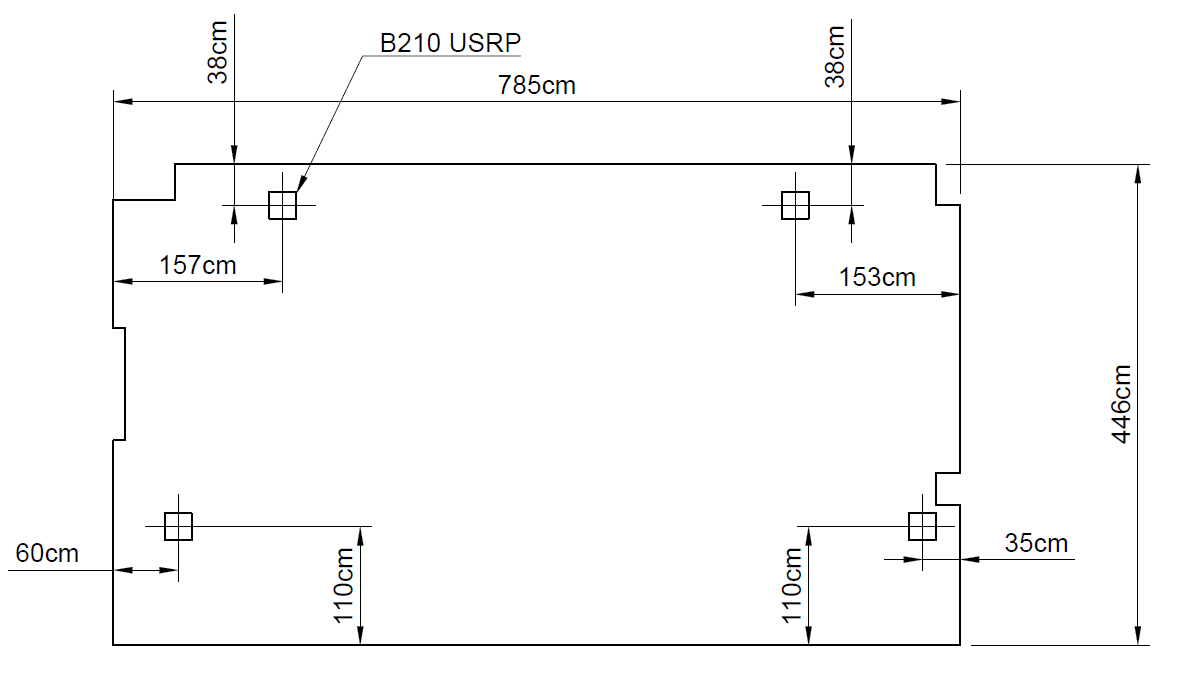
\includegraphics[width=1\linewidth]{src//img/room117tesbed.png}
    \caption{Radio Testbed Layout}
    \label{fig:appendix:testbed-drawing}
\end{figure}

\section{Software Stack}
There are multiple software artefacts needed to run the testbed. To run the base stations, srsRAN's eNB code is used to control the USRPs that host the radio layer of the network. For (\todo{add reasons}), we use open5gs to run the network core, which is responsible for authenticating users, orchestrating the network and providing a control flow. A Kubernetes \insertref deployment is used to run all of these simultaneously, nominating the base stations and core network as pods and the physical NUCs and clusters as the nodes. The exact tools were used with generous permission from Jon Larrea [https://orcid.org/0000-0001-5736-2107], the author of the deployment tools.

\todo{Add a figure here maybe?}

\section{UE setup}
\tocomplete{Finish UE setup}
\begin{itemize}
    \item The phone
    \item The laptop
\end{itemize}
